

\section{Background}\label{sec:background}

In this section, we present the background of SSD internals (Section~\ref{sec:SSDInternals}) and Lucene's architectures (Section~\ref{sec:searchEngineArch}).

\subsection{Modern SSDs}\label{sec:SSDInternals}

\begin{figure}[htbp]
  \centering
  \begin{tabular}{ccc}
 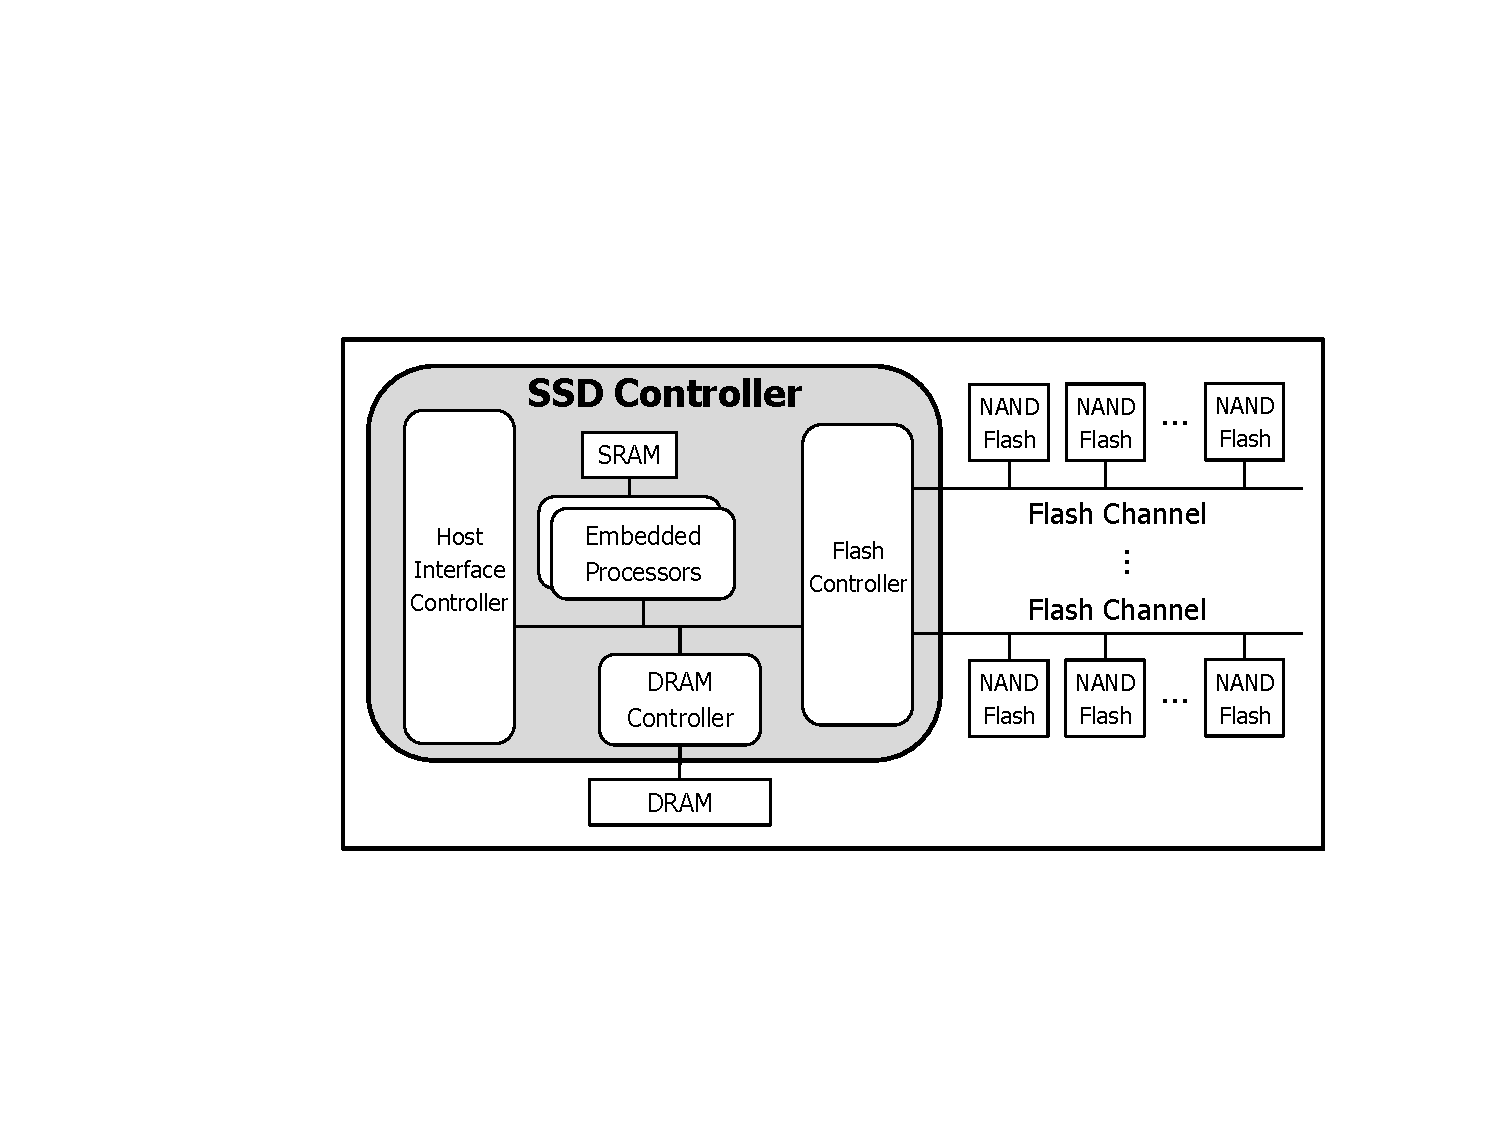
\includegraphics[width=0.95\columnwidth]{figures/SSDInternals.pdf}
\end{tabular}
  \caption{SSD internals}
  \label{fig:SSDInternals}
 \end{figure}

Figure~\ref{fig:SSDInternals} represents a typical modern SSD and its main components. In general, an SSD is largely composed of NAND flash memory array, SSD controller, and DRAM. The SSD controller subdivides into four main subcomponents such as host interface controller, embedded processors, DRAM controller, and flash memory controller.

Commands come from a user through the host interface and the most common interfaces, for instance, Serial ATA (SATA), Serial Attached SCSI (SAS), or PCI Express (PCIe), are implemented by the host interface controller.
The embedded processors in the SSD controller receive the commands and pass them to the flash memory controller. They, more importantly, run SSD firmware codes for computation and execute Flash Translation Layer (FTL) for logical-to-physical address mapping. Typically, modern SSD is equipped with a low-powered 32-bit processor such as an ARM Cortex series processor. Each processor can have a tightly coupled memory (e.g., SRAM) for the purpose of even faster access to frequently accessed data or codes. Each processor can access DRAM through the DRAM controller. For data transfer between flash memory and DRAM, the Flash Controller, also called Flash Memory Controller (FMC), is adopted. The FMC runs Error Correction Codes (ECC) and supports Direct Memory Access (DMA) functionality.

%The NAND flash memory package (also called chip) is persistent storage media and each package consists of one or more dies. The die is the smallest unit that can independently execute commands or report status. Each die contains one or more planes (usually one or two). Identical or concurrent operations can take place on each plane, although with some restrictions. Each plane subdivides into a number of blocks which are the smallest erase unit, and finally each block is composed of many pages (typically 64 or 128 pages)which are the smallest read/write unit.
The NAND flash memory package (also called chip) is persistent storage media and each package subdivides further into smaller units that can independently execute commands or report status. An SSD is also equipped with a large size of DRAM for buffering data or storing metadata of the address mapping. All the flash channels share access to the DRAM. Thus, data transfer from the flash channels to the DRAM needs to be serialized.


\subsection{Query Processing of Lucene}\label{sec:searchEngineArch}

\begin{figure}[htbp]
  \centering
  \begin{tabular}{ccc}
 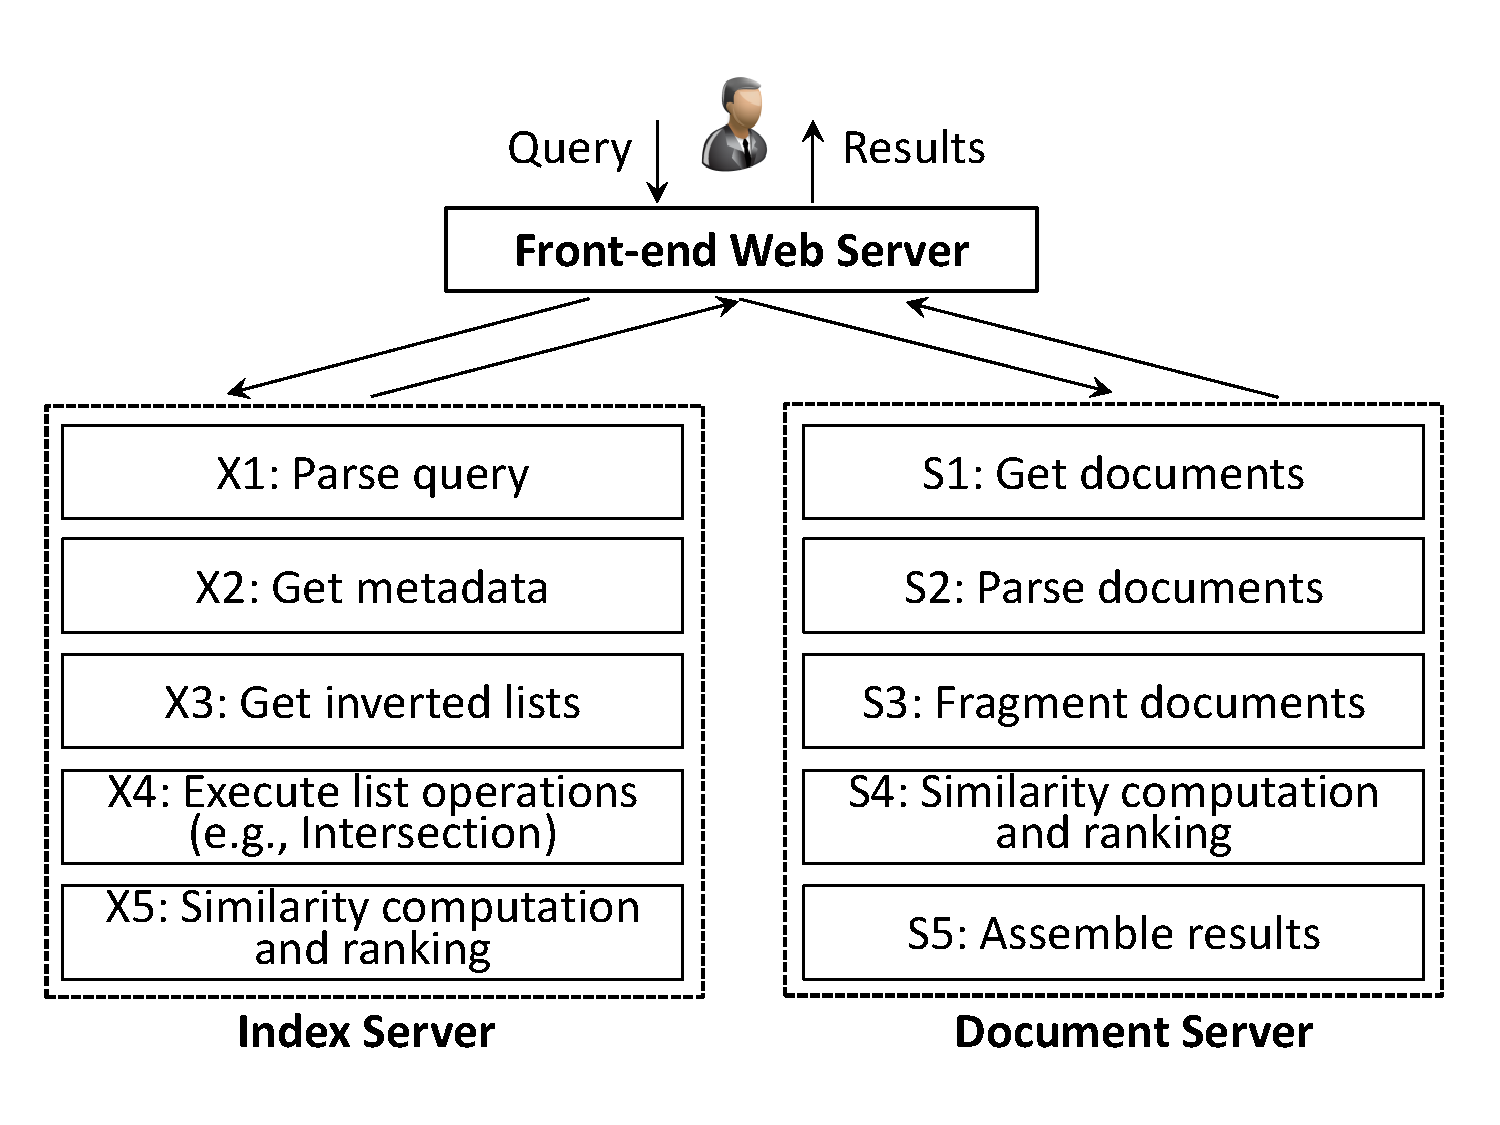
\includegraphics[width=0.5\columnwidth]{figures/searchEngineArch.pdf}
\end{tabular}
  \caption{Query processing of Lucene}
  \label{fig:searchEngineArch}
 \end{figure}

Lucene is a well known open-source search engine and widely adopted in industry. E.g., LinkedIn~\cite{Hien2013} and and Twitter~\cite{Busch2012ERS} adopted Lucene in their search platforms.

%We provide some background of how a query is executed in Lucene. 
Like other search engines, Lucene relies on the standard inverted index \cite{ZM06} to answer user queries efficiently. The inverted index is essentially a mapping data structure of key-value pairs, where the key is a query term, the value is a list of documents containing the term.

Upon receiving a user query $q$ (e.g., ``SSD database''), Lucene answers it through several steps (S1 to S5 in Figure~\ref{fig:searchEngineArch}).
By default, Lucene enables \texttt{AND} query mode (unless users explicitly specify other query modes, e.g., \texttt{OR}, \texttt{NOT}), which returns a list of documents that contain \emph{all} of the query terms.
 
\emph{Step S1}: parse the query to a parse tree (similar to the parse tree in SQL queries). The query $q$ will be tokenized into several query terms. In our example, it has two query terms: ``SSD'' and ``database''.
%Each node is a Lucene-defined query type. The root node is a conjunction query. Each leaf node is a term query.
%Each node is a Lucene-defined query type. The root node is a conjunction query, which returns the intersected results returned by the leaf nodes. Each leaf node is a term query, which returns a list of documents that contain that term, by referring to the inverted index.
\textit{Step S2}: get metadata for each query term. The metadata is used to load the inverted list of each query term in the following step. Thus, this metadata stores some basic information about the on-disk inverted list. In Lucene, it contains (1) the offset where the list is located on disk, (2) the list length (in bytes), and (3) the number of entries in the list.
\textit{Step S3}: for each term, get the inverted list from disk to memory.
\textit{Step S4}: execute list operations depending on query modes. In our example, it is intersection (because of the \texttt{AND} query mode). It could be other operations such as union (\texttt{OR} mode) or difference (\texttt{NOT} mode).
\textit{Step S5}: for each qualified document $d$, calculate the similarity value between the query $q$ and the document $d$ by using an IR relevance model. Lucene adopts a modified BM25 model~\cite{Robertson1994}. Finally, Lucene returns top-ranked results to end users.

We note that Lucene may not embrace all state-of-the-art query processing techniques. For instance, both step S4 and S5 may be able to be algorithmically combined for early termination~\cite{Broder2003EQE,Fagin2001}.

